\chapter{Литературный обзор} \label{chapt1}

\section{Гексагональный нитрид бора} \label{sect1_1}
Примерами классических квази-2D-структур являются слоистые кристаллы.
Изучение таких кристаллов началось еще в конце сороковых годов
двадцатого века~\cite{Wallace1947} и продолжается по сей день.
Наиболее интересными представителями таких систем являются кристаллы
гексагонального нитрида бора и графита. В настоящей работе исследовался
именно гексагональный нитрид бора.
\subsection{Кристаллическая структура} \label{sect1_3_1}
Нитрид бора существует в различных модификациях: ромбоэдрический нитрид
бора(g-BN), кубический нитрид бора(c-BN)~\cite{Litvinov1998},
вюрцитный нитрид бора($\omega$-BN) и гексагональный нитрид бора
(h-BN) рис.~\ref{pic:BN_forms}. Также нитрид бора может существовать в виде нанотрубок~\cite{YZhi2009}
и фуллеренов.
\begin{figure}[!ht]
\center{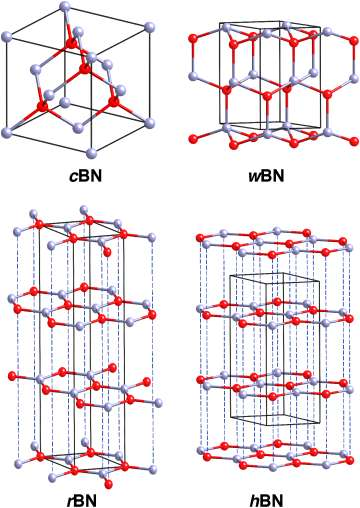
\includegraphics[width=0.4\linewidth]{BN_forms.png}}
\caption{cBN - кубический нитрид бора, wBN - вюрцитный нитрид бора,
rBN - ромбоэдрический нитрид бора, hBN - гексагональный нитрид бора}
\label{pic:BN_forms}
\end{figure}


Гексагональный нитрид бора является наиболее стабильной формой нитрида
бора и представляет собой слоистую структуру, подобную графиту~\cite{
Neumann1995,Doni1969}. В спрессованном состоянии h-BN обладает 
полупроводниковыми свойствами, а присутствие примесей в соединении 
может вызывать люминесценцию. В связи с этим гексагональный нитрид 
бора интересен областью применения как в цветной металлургии, 
благодаря своей химической инертности и антиадгезионным свойствам по 
отношению к металлам и сплавам,так и в полупроводниковой 
промышленности, благодаря широкой запрещенной зоне~\cite{
Serzhantova2011}.




















